\documentclass{esg8022pset}
\begin{preamble}
  \usepackage{amsmath}
  \usepackage{amssymb}
  \usepackage{enumerate}
  \usepackage{graphicx}
  \usepackage{hyperref}
  \usepackage{mathtools}
  \usepackage[per-mode=symbol]{siunitx} %If this line is giving you trouble, try replacing per-mode with per
  \providecommand{\uvec}[1]{{\hat{\bf{#1}}}}
  \usepackage{pgf,tikz}
  \usetikzlibrary{arrows}
  \usepackage{wasysym}
  \usepackage{subfig}
  \makeatletter
  \newcommand{\interitemtext}[1]{%
    \begin{list}{}
     {\itemindent=0mm\labelsep=0mm
     \labelwidth=0mm\leftmargin=0mm
     \addtolength{\leftmargin}{-\@totalleftmargin}}
      \item #1
    \end{list}
  }
  \makeatother
  \renewcommand{\d}{\,d}
  \providecommand{\norm}[1]{\lVert#1\rVert}
  
  \newcommand{\Kgrad}{\left(\hat{x} \frac{\partial}{\partial x} + \hat{y} \frac{\partial}{\partial y} + \hat{z} \frac{\partial}{\partial z}\right)}
  \newcommand{\Kdiv}[6]{{#4}\left(\frac{\partial {#1}}{\partial x} {#5} \frac{\partial {#2}}{\partial y} {#6}\frac{\partial #3}{\partial z} \right)}
  \newcommand{\KKdiv}[6]{{#4}\left(\frac{\partial}{\partial x}{#1} {#5} \frac{\partial}{\partial y}{#2} {#6}\frac{\partial}{\partial z}{#3} \right)}
  \newcommand{\dx}{\frac{\partial}{\partial x}}
  \newcommand{\dy}{\frac{\partial}{\partial y}}
  \newcommand{\dz}{\frac{\partial}{\partial z}}
  \newcommand{\dtheta}{\frac{\partial}{\partial \theta}}
  \newcommand{\dr}{\frac{\partial}{\partial r}}
  
  \AtBeginDocument{%
    % Appologies to any future editor on the inconsistencies in TeX code and the unnecessary braces.  I'm aggregating previously typeset problems, and didn't think it worth my time to improve the quality of TeX code in ways that won't make any difference to the typeset material. -Jason Gross (jgross@mit.edu)
  }%
\end{preamble}

\classname{Physics 8.022}
\semester{Spring 2011}
\problemsetnumber{4}
\duedate{Sunday, February 27 at 10 \textsc{pm}}
%\readingassignment{Kleppner and Kolenkow, \emph{An Introduction to Mechanics}, Chapters Seven and Eight}
\problemsettitle{Conductors and Capacitors}

\begin{document}

\begin{problem}{Purcell 3.1: Charges in a spherical conductor}
  A spherical conductor $A$ contains two spherical cavities. The
  total charge on the conductor itself is zero. However, there is a
  point charge $q_b$ at the center of one cavity and $q_c$ at the
  center of the other.  A considerable distance $r$ away is another
  charge $q_d$. What force acts on each of the four objects, $A$,
  $q_b$, $q_c$, $q_d$? Which answers, if any, are only approximate,
  and depend on $r$ being relatively large?
  \begin{center}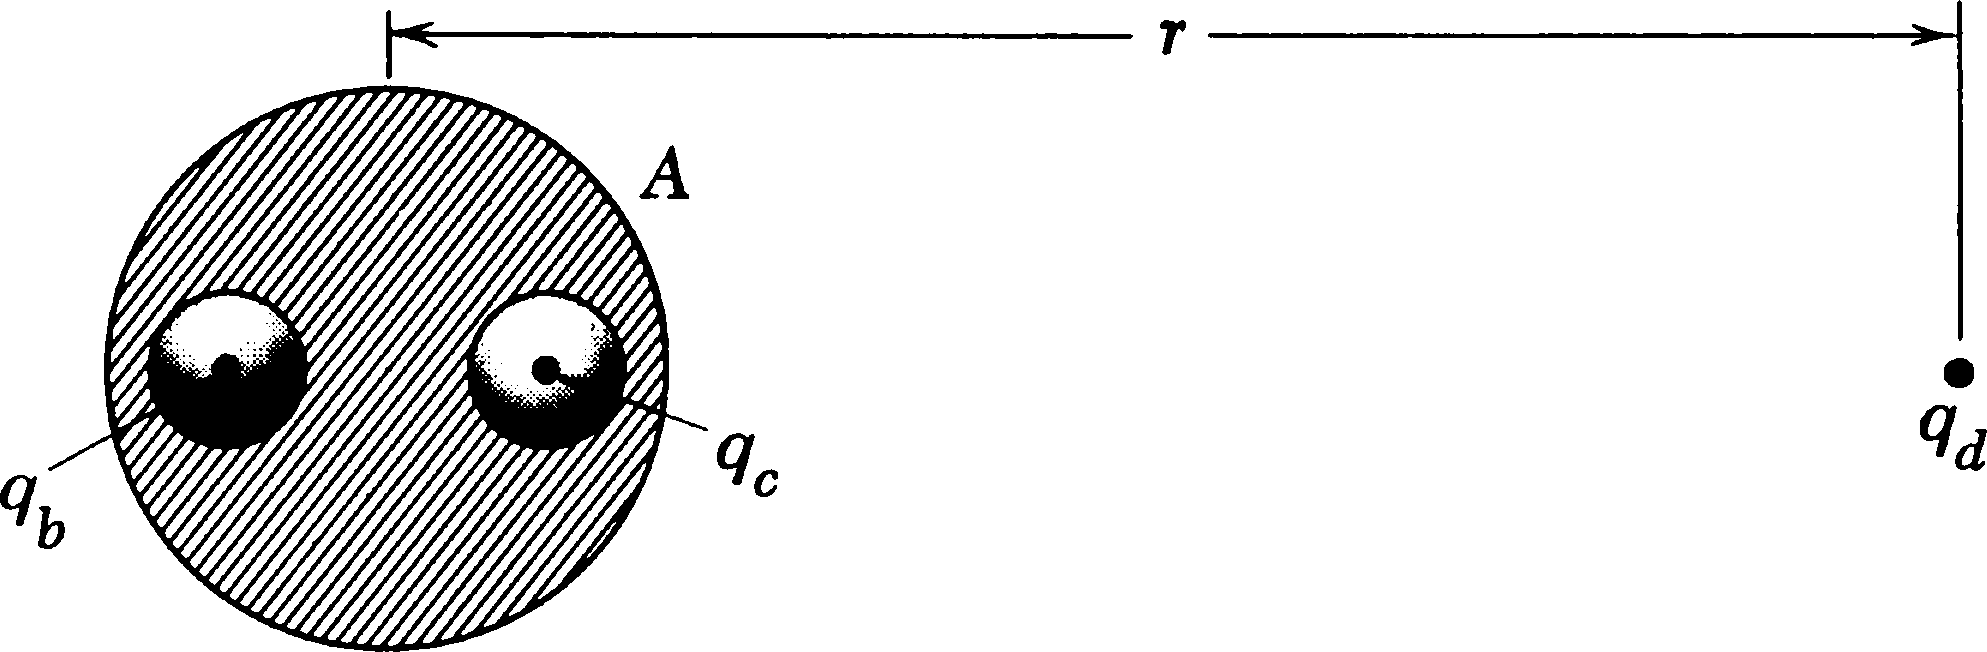
\includegraphics[width=0.5\textwidth]{ps04_01}\end{center}
\end{problem}
\begin{solution}

\end{solution}


\begin{problem}{Purcell 3.3: Charge over the plane} 
  In the field of a point charge over the plane (Fig. 3.9), if you
  follow a field line that starts out from the point charge in a 
  horizontal direction, that is, parallel to the plane, where does
  it meet the surface of the conductor?
  
  \textbf{Figure 3.9} Some field lines for the charge above the plane. 
  The field strength at the surface, given by the equation below,
  determines the surface charge density $\sigma$. 
  \begin{center}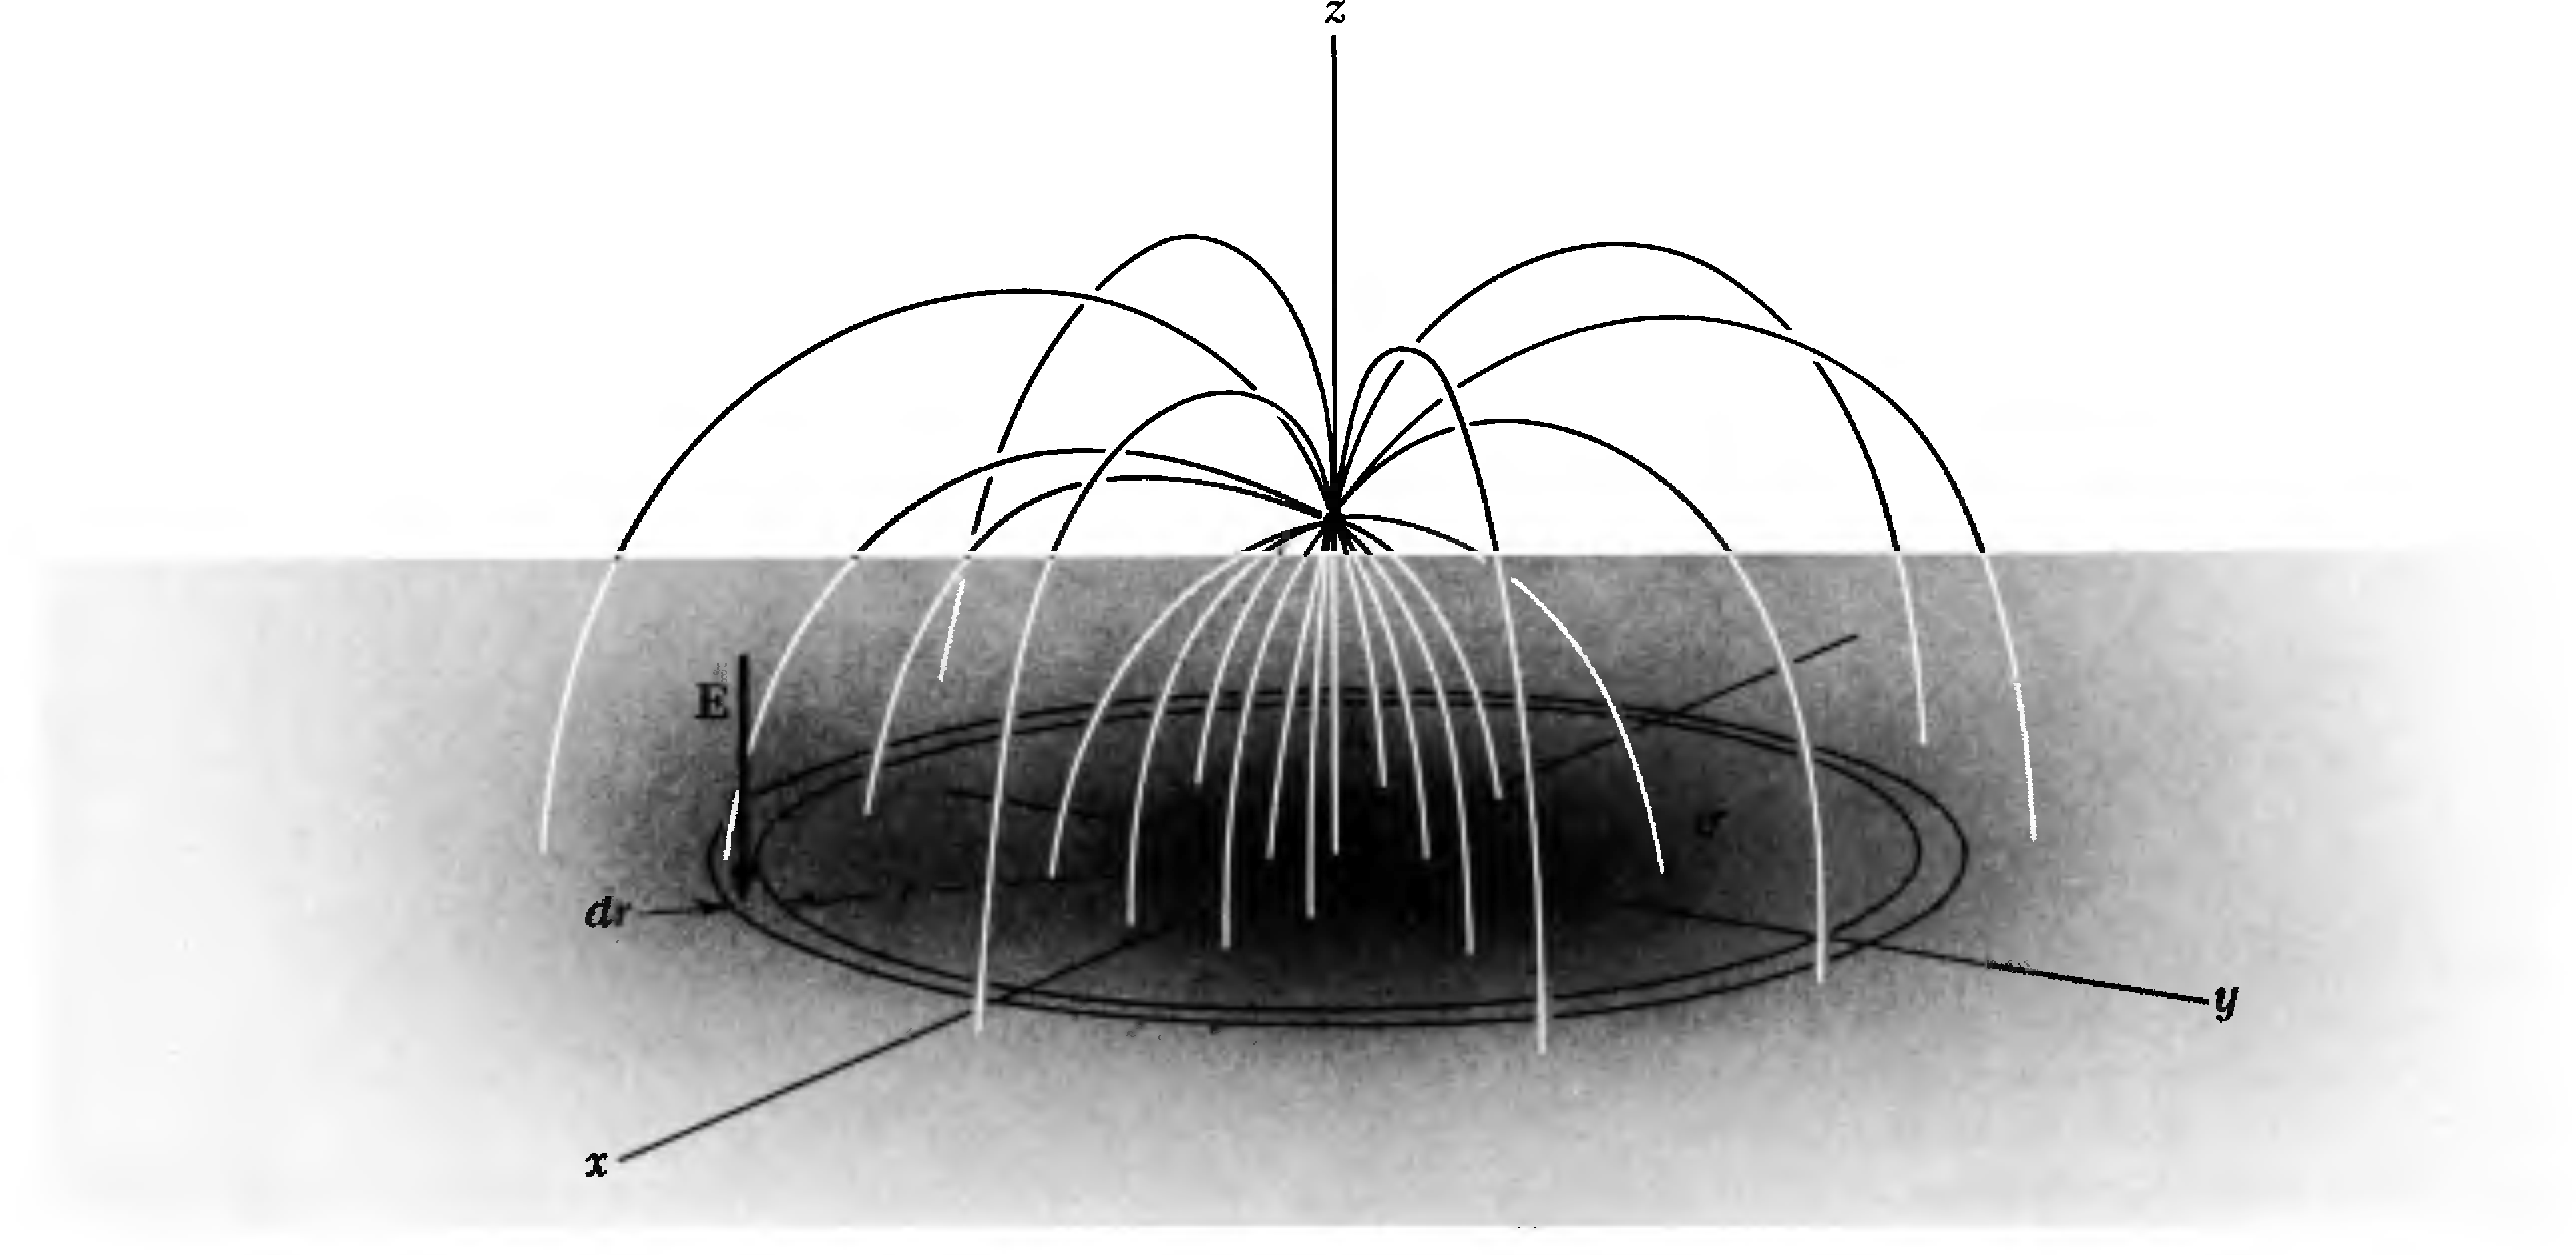
\includegraphics[width=0.5\textwidth]{ps04_02}\end{center}
  \begin{equation*}
    E_z = \frac{-2Q}{r^2 + h^2} \cos\theta = \frac{-2Q}{r^2 + h^2}\cdot \frac{h}{(r^2 + h^2)^{1/2}} = \frac{-2Qh}{(r^2 + h^2)^{3/2}}
  \end{equation*}
  
  \noindent \textsc{Hint}: Sketch the field lines in question.  Draw 
  a Gaussian surface that is just barely inside those lines.  Close 
  off the bottom.  You should have a closed surface that looks like 
  an inverted bowl.  What is the total charge contained within this 
  surface?  Now compute the total flux through this closed surface:
  How much goes through the top, curved portion of the inverted bowl?
  How much goes through the bottom, right next to the conducting plane?
\end{problem}
\begin{solution}

\end{solution}



\begin{problem}{Purcell 3.5: Work pulling a charge away from a conducting plane}
  A charge $Q$ is located $h$ cm above a conducting plane, just as
  in Fig. 3.8a. Asked to predict the amount of work that would have
  to be done to move this charge out to infinite distance from the
  plane, one student says that it is the same as the work required to
  separate to infinite distance two charges $Q$ and $-Q$ which are
  initially $2h$ cm apart, hence $W = Q^2 / 2h$. Another student
  calculates the force that acts on the charge as it is being moved
  and integrates $F \d x$, but gets a different answer. What did the
  second student get, and who is right?
  \begin{center}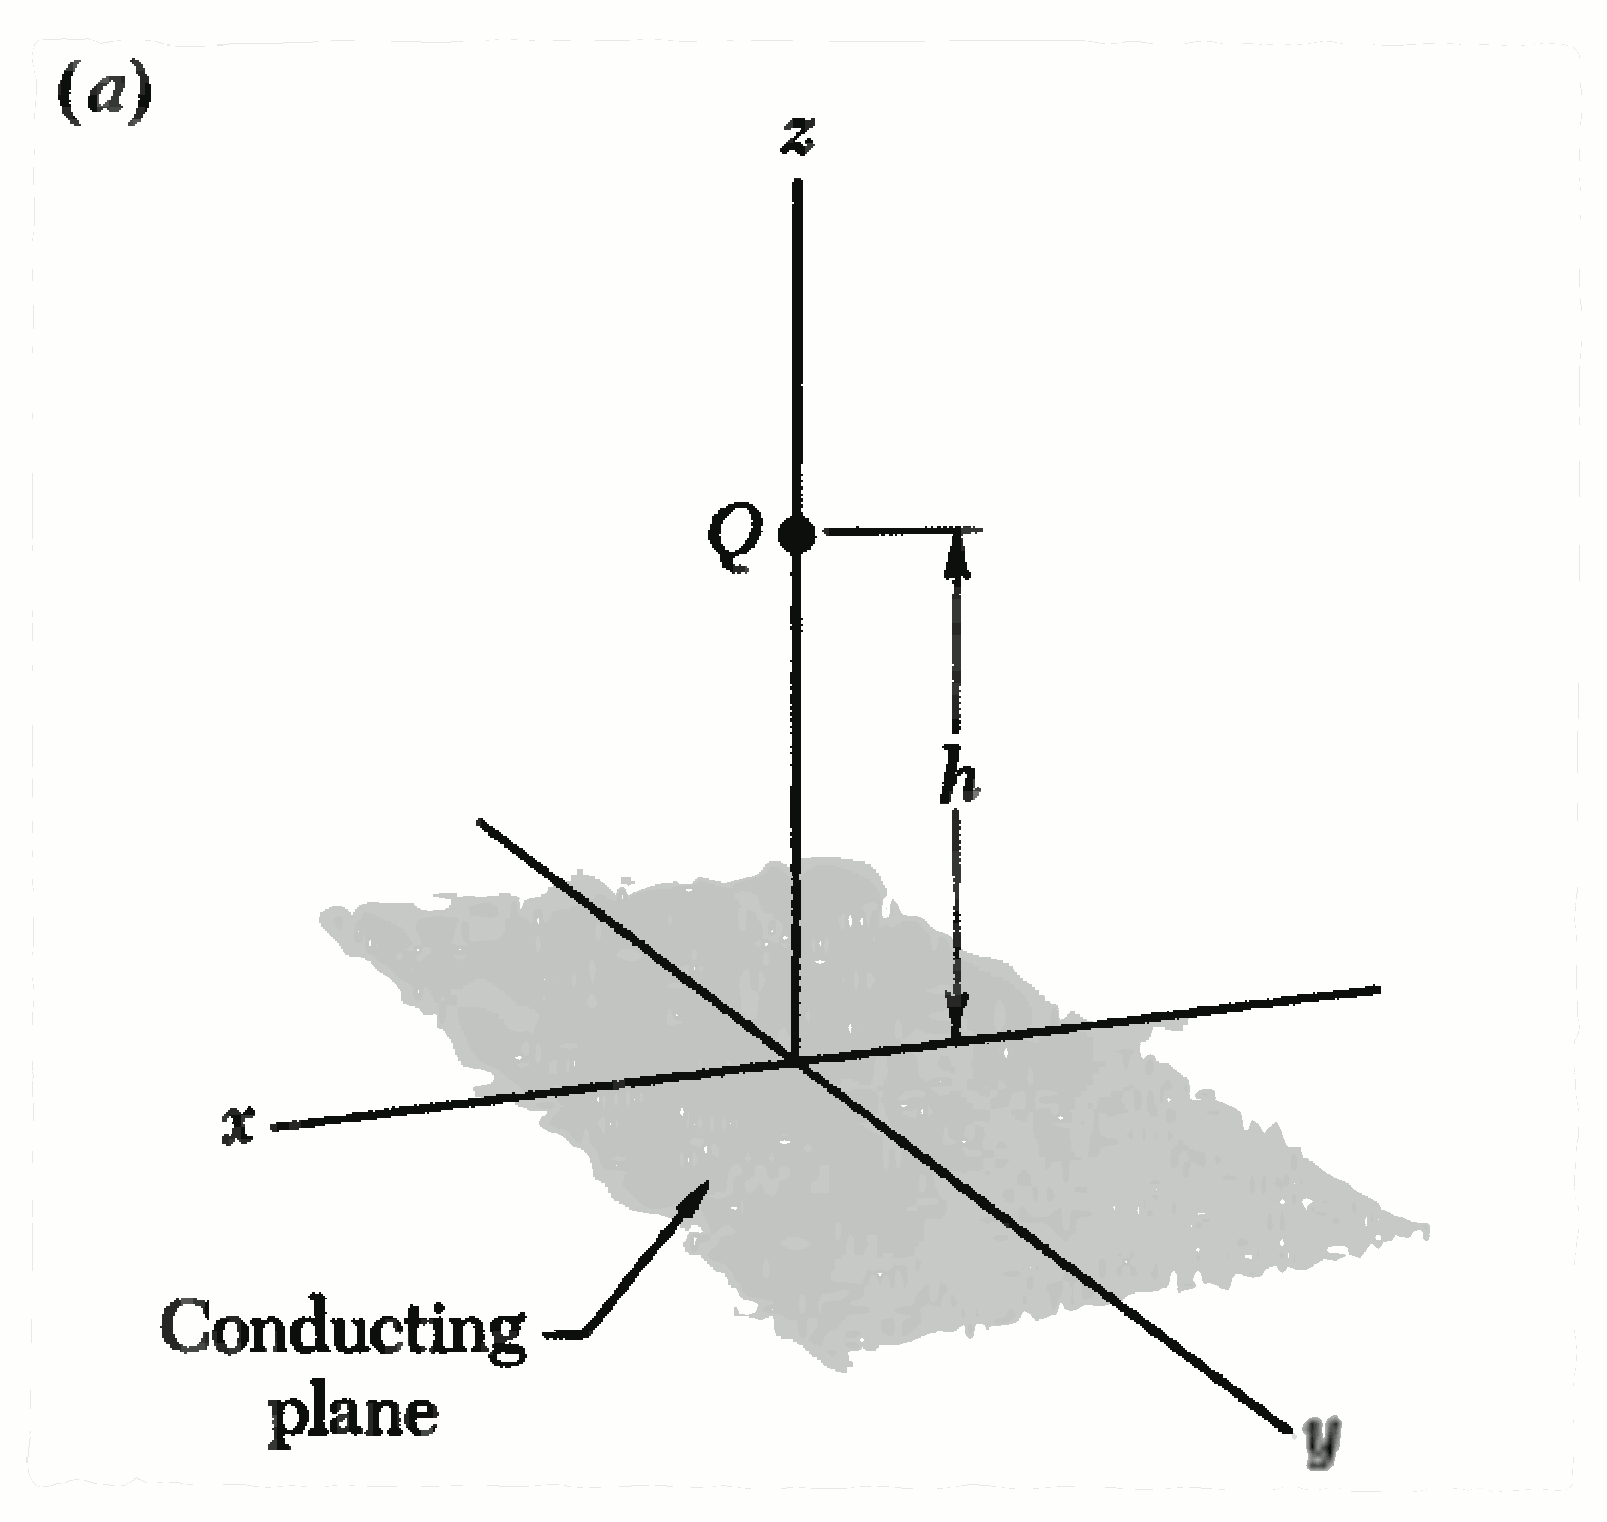
\includegraphics[width=0.5\textwidth]{ps04_03}\end{center}
\end{problem}
\begin{solution}
  
\end{solution}








\begin{problem}{Purcell 3.8: Three conducting plates}
  Three conducting plates are placed parallel to one another as
  shown. The outer plates are connected by a wire. The inner plate
  is isolated and carries a charge amounting to 10 esu per square
  centimeter of plate. In what proportion must this charge divide
  itself into a surface charge $\sigma_1$ on one face of the inner
  plate and a surface charge $\sigma_2$ on the other side of the
  same plate?
  \begin{center}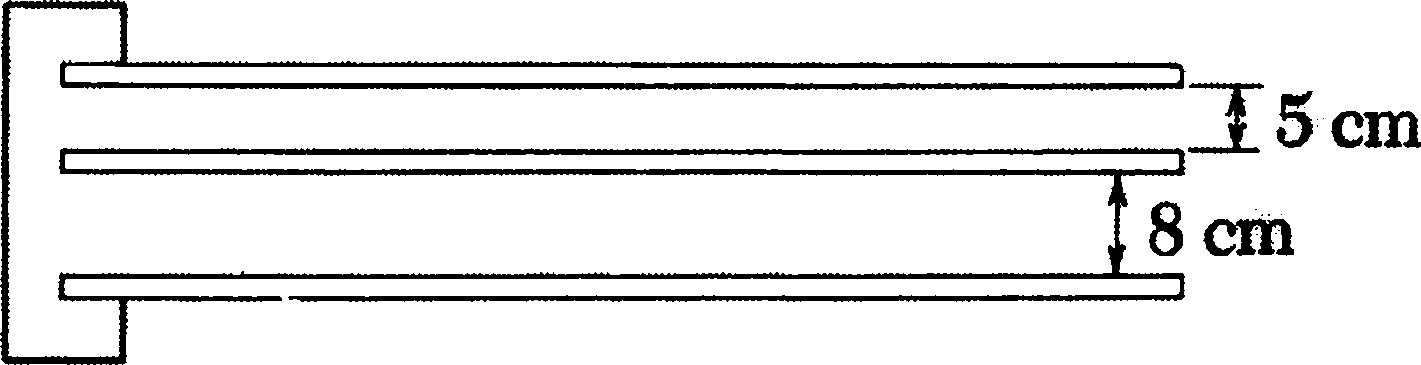
\includegraphics[width=0.5\textwidth]{ps04_04}\end{center}
\end{problem}
\begin{solution}

\end{solution}





\begin{problem}{Purcell 3.17: Design a spherical capacitor}
  We want to design a spherical vacuum capacitor with a given
  radius $a$ for the outer sphere, which will be able to store the greatest 
  amount of electrical energy subject to the constraint that the electric 
  field strength at the surface of the inner sphere may not exceed $E_0$. 
  What radius $b$ should be chosen for the inner spherical conductor, and 
  how much energy can be stored? 
  
  \begin{flushright}\emph{Ans}. $\frac34 a$; $\frac{27}{512} a^3 E_0^2$.\end{flushright}
\end{problem}
\begin{solution}
  
\end{solution}





\begin{problem}{Purcell 3.19: Semicylindrical electrodes}
  In the apparatus shown, ions are accelerated through a potential difference $V_0$ and then enter the space between the semicylindrical electrodes $A$ and $B$. Show that an ion will follow the semicircular path of radius $r_0$ if the potentials of the outer and inner electrodes are maintained, respectively, at $2V_0\ln(b/r_0)$ and $2V_0\ln(a/r_0)$. (The cylindrical electrodes $A$ and $B$ are assumed to be long, in the direction perpendicular to the diagram, compared with the space between them.) 
  \begin{center}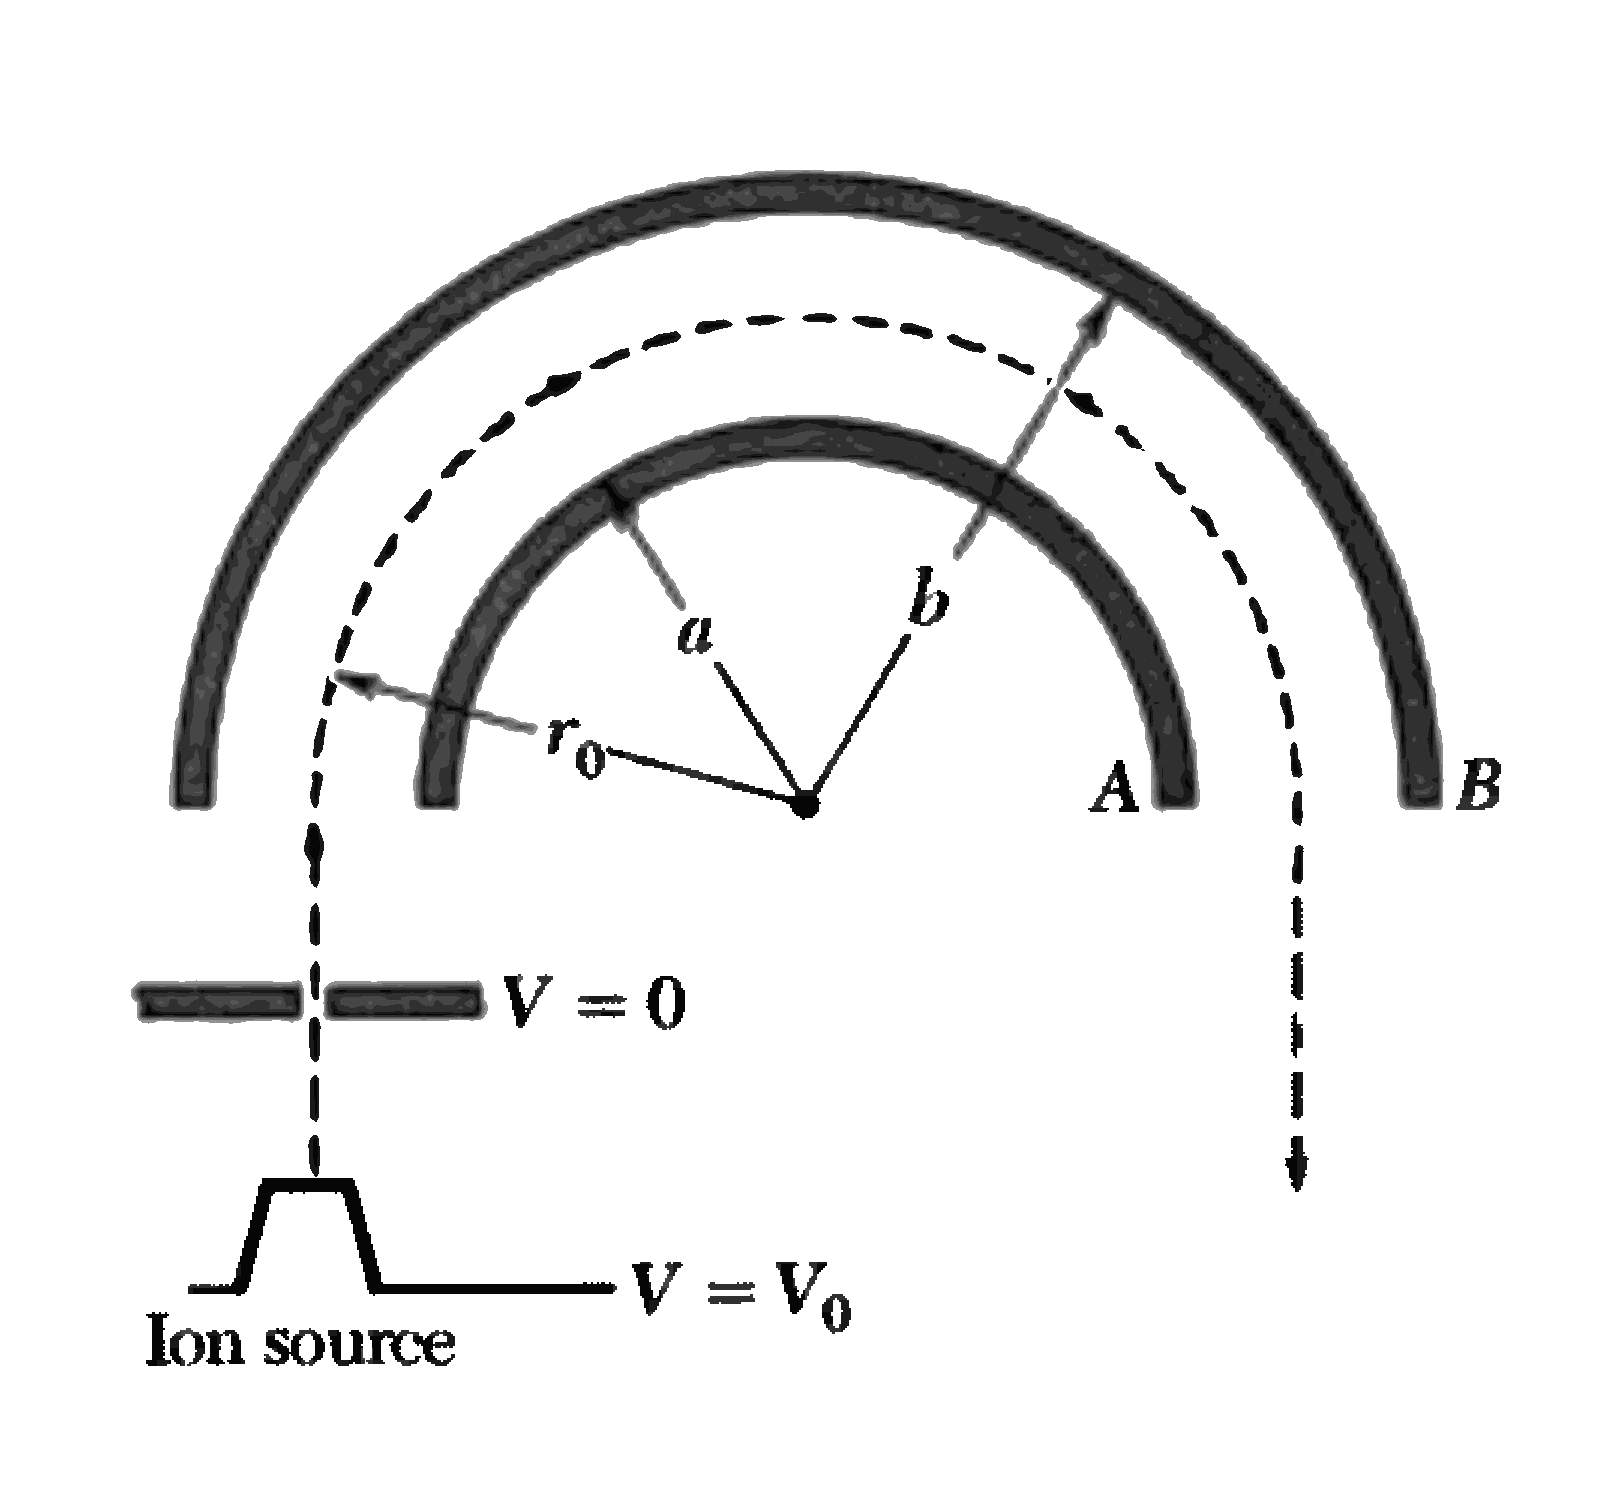
\includegraphics[width=0.5\textwidth]{ps04_06}\end{center}
\end{problem}
\begin{solution}

\end{solution}





\begin{problem}{Purcell 10.1: Make a capacitor}
  \begin{enumerate}[(a)]
    \item You have a supply of polyethylene tape, dielectric constant 
      2.3, 2.25 inches wide, and 0.001 inch thick; also, a supply of aluminum 
      tape 2 inches wide and 0.0005 inch thick. You want to make a capacitor
      of about 0.05 microfarad capacitance, in the form of a compact 
      cylindrical roll. Describe how you might do this, estimating the 
      amount of tape of each kind that would be needed, and the overall 
      diameter of the finished capacitor. 
    \item (Optional --- Group Challenge) Build a Leyden jar, charge it
      and determine how much charge it stores. Be creative!  You can ask
      Paola and the TAs for hints.
  \end{enumerate}
\end{problem}
\begin{solution}

\end{solution}






\begin{problem}{Purcell 10.14: Capacitors with a dielectric}
  The figure shows three capacitors of the same area and plate 
  separation. Call the capacitance of the vacuum condenser $C_0$. Each of 
  the others is half-filled with a dielectric, with the same dielectric constant
  $k_e$, but differently disposed, as shown. Find the capacitance of 
  each of these two capacitors. (Neglect edge effects.)
  \begin{center}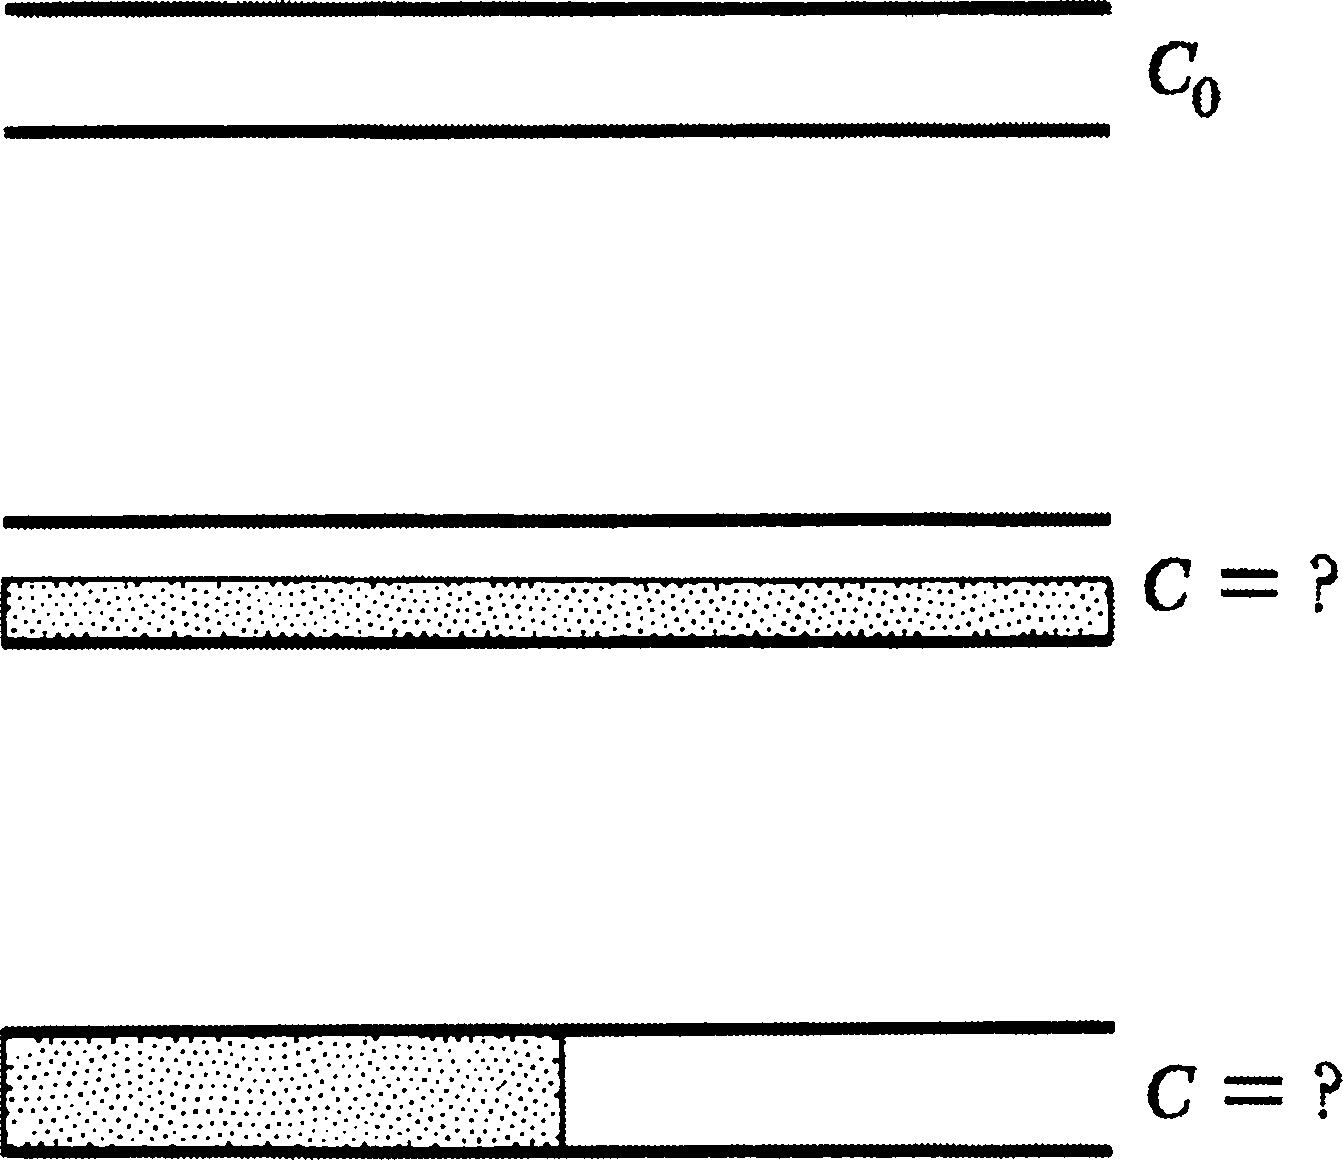
\includegraphics[width=0.33\textwidth]{ps04_08}\end{center}
\end{problem}
\begin{solution}

\end{solution}





\begin{problem}{Purcell 10.6: ``Fringing'' field far away from a parallel-plate capacitor}
  A parallel-plate capacitor, with a measured capacitance $C = \SI{250}{\centi\meter}$,
  is charged to a potential difference of 6 statvolts. The plates 
  are \SI{1.5}{\centi\meter} apart. We are interested in the field outside the capacitor,
  the ``fringing'' field which we usually ignore. In particular, we would 
  like to know the field at a distance from the capacitor large compared 
  with the size of the capacitor itself. This can be found by treating the 
  charge distribution on the capacitor as a dipole. Estimate the electric 
  field strength 
  \begin{enumerate}[(a)]
    \item At a point 3 meters from the capacitor in the plane of the plates. 
    \item At a point the same distance away, in a direction perpendicular to the plates. 
  \end{enumerate}
\end{problem}
\begin{solution}

\end{solution}

\end{document}
